\documentclass[conference]{IEEEtran}
\IEEEoverridecommandlockouts
\usepackage{cite}
\usepackage[utf8]{inputenc}
\usepackage[T1]{fontenc}
\usepackage[spanish,es-tabla]{babel}
\usepackage{amsmath,amssymb,amsfonts}
\usepackage{graphicx}
\usepackage{booktabs}
\usepackage{textcomp}
\usepackage{xcolor}
\usepackage{url}

% Marcador de pendientes: se ve en rojo en el PDF. Buscar "TODO" antes de enviar.
\newcommand{\todo}[1]{\textcolor{red}{[TODO: #1]}}

\begin{document}

\title{Reducción del número de mediciones en una cámara de un píxel:\\
patrones y reconstrucción en 2D sobre vistas de escenas 3D}

\author{\IEEEauthorblockN{Francisco Alfaro}
\IEEEauthorblockA{\textit{Departamento de Electrónica} \\
\textit{Universidad Técnica Federico Santa María}\\
Valparaíso, Chile \\
francisco.alfaro@usm.cl}
\and
\IEEEauthorblockN{Ayrton Perez}
\IEEEauthorblockA{\textit{Departamento de Informática} \\
\textit{Universidad Técnica Federico Santa María}\\
Valparaíso, Chile \\
ayrton.perez@usm.cl}
}

\maketitle

\begin{abstract}
Una cámara de un píxel (Single Pixel Camera, SPC) reemplaza el sensor matricial por un detector único y una
secuencia de patrones de iluminación, lo que abarata el sensor a cambio de más mediciones por imagen. Este trabajo
estudia cuánta calidad se pierde al reducir esas mediciones cuando las imágenes son vistas de una escena 3D, como paso
previo a su reconstrucción con 3D Gaussian Splatting. Se simula la adquisición sobre 24 vistas de cada una de cuatro
escenas de Tanks and Temples y Deep Blending, con patrones Hadamard ordenados y binarios aleatorios, un modelo de
detector con ruido de Poisson, ruido de lectura y cuantización de 16 bits, y se comparan la reconstrucción directa y la
regularizada con variación total. Con Hadamard y variación total, la calidad media crece de 28.1 dB (PSNR) con el 5 \% de
las mediciones a 34.6 dB con el 50 \%, y la regularización aporta entre 1.8 y 2.1 dB sobre la reconstrucción directa. Los
patrones aleatorios sin regularización fallan (13.6 a 17.1 dB), pero con regularización se acercan a Hadamard a razones
altas. El alcance se limita al caso 2D; la propagación del error a la escena 3D se deja como trabajo futuro. El código
está disponible públicamente.
\end{abstract}

\begin{IEEEkeywords}
single pixel camera, Hadamard, muestreo comprimido, variación total, 3D Gaussian splatting
\end{IEEEkeywords}

\section{Introducción}
Las cámaras de un píxel miden proyecciones de la escena sobre patrones codificados y reconstruyen la imagen resolviendo
un problema inverso \cite{duarte2008,edgar2019}. Son atractivas donde fabricar un sensor matricial es costoso, por
ejemplo en bandas espectrales poco habituales, pero cada imagen exige una secuencia de mediciones.

Ese costo se multiplica cuando el objetivo es una escena 3D. Métodos recientes como NeRF \cite{mildenhall2020} y 3D
Gaussian Splatting (3DGS) \cite{kerbl2023} necesitan cientos de vistas, de modo que cada medición ahorrada por vista
reduce de forma importante el tiempo total de captura. La pregunta de este trabajo es cuántas mediciones por vista se
pueden quitar antes de que la calidad caiga, y qué patrón y qué reconstrucción lo soportan mejor.

\textbf{Contribuciones.} (i) Una simulación SPC a resolución cercana a la nativa, con una transformada rápida de
Walsh-Hadamard en GPU y un modelo explícito del detector. (ii) Una comparación de patrones (Hadamard ordenado y binario
aleatorio) y de reconstrucción (directa y con variación total) sobre cuatro escenas. (iii) Estudios de ruido, de orden
de patrones y de color. (iv) El código abierto de todo el flujo.

\textbf{Alcance.} Este artículo cubre únicamente la adquisición y reconstrucción en 2D. El entrenamiento de 3DGS con
las vistas reconstruidas está implementado en el repositorio, pero sus resultados quedan fuera de este trabajo.

\section{Trabajo relacionado}
\subsection{Cámara de un píxel y muestreo comprimido}
La arquitectura de imagen comprimida con un microespejo digital (DMD) y un fotodiodo se debe a Takhar y Wakin
\cite{takhar2006,wakin2006}, y Duarte et al.\ \cite{duarte2008} la formalizaron como cámara de un píxel. Se apoya en la
teoría de muestreo comprimido \cite{donoho2006,candes2006}, que permite recuperar señales escasas con pocas
mediciones. Edgar et al.\ \cite{edgar2019} ofrecen una revisión del campo, y Sun et al.\ \cite{sun2013} llevaron la
idea a imagen 3D con varios detectores.

\subsection{Patrones: Hadamard, Fourier y su orden}
Zhang et al.\ \cite{zhang2017hadfourier} comparan las bases de Hadamard y de Fourier. Con una base completa, el orden en
que se miden los patrones decide qué información se captura primero: el orden \textit{Russian dolls}
\cite{sun2017russian} y el \textit{cake-cutting} \cite{yu2019cake} priorizan las bajas frecuencias para lograr
reconstrucciones sub-Nyquist.

\subsection{Reconstrucción de escenas 3D}
NeRF \cite{mildenhall2020} representa la escena con un campo neuronal, y 3DGS \cite{kerbl2023} con millones de
gaussianas 3D optimizadas a partir de imágenes y poses estimadas con Structure from Motion \cite{schonberger2016}.
La Fig.~\ref{fig:3dgs} resume el renderizado. Se evalúan sobre Tanks and Temples \cite{knapitsch2017} y Deep Blending \cite{hedman2018}, los mismos conjuntos que se
usan aquí.

\begin{figure}[t]
\centering
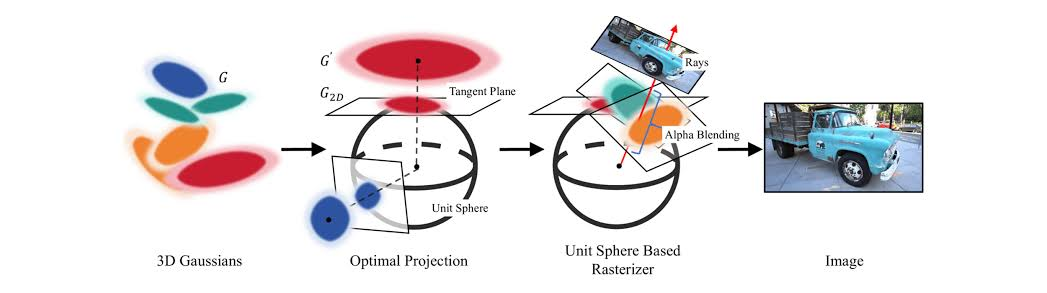
\includegraphics[width=\columnwidth]{figs/3dgs.jpeg}
\caption{Renderizado de 3DGS: gaussianas 3D, proyección al plano de la imagen, mezcla alfa e imagen resultante (variante con proyección sobre la esfera unitaria). \todo{verificar y citar la fuente de la figura}}
\label{fig:3dgs}
\end{figure}

\section{Modelo de medición}
Sea $\mathbf{x}\in\mathbb{R}^{N}$ una vista vectorizada, con $N=H\times W$. La SPC (Fig.~\ref{fig:spc}) mide
\begin{equation}
\mathbf{y}=\mathbf{\Phi}\mathbf{x}+\mathbf{n},\qquad \mathbf{\Phi}\in\mathbb{R}^{M\times N},
\label{eq:medicion}
\end{equation}
con razón de medición $r=M/N$. Un DMD solo implementa máscaras $\{0,1\}$, de modo que se miden los patrones
$\mathbf{P}=(\mathbf{1}+\mathbf{H})/2$ y una medición adicional de nivel DC (todos los espejos encendidos); el
coeficiente en $\pm1$ se recupera como $c=2y-\text{DC}$, lo que duplica la amplitud del ruido. La alternativa diferencial (Fig.~\ref{fig:diferencial}) mide por separado los patrones positivo y negativo y requiere el doble de mediciones.

\begin{figure}[t]
\centering
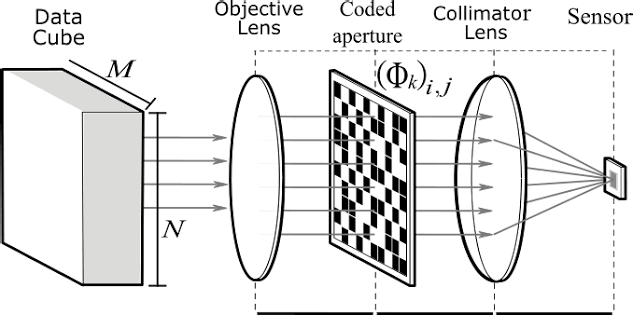
\includegraphics[width=0.95\columnwidth]{figs/single-pixel.png}
\caption{Arquitectura de una cámara de un píxel: la escena atraviesa una apertura codificada con el patrón $\Phi_k$ y un único sensor mide la suma. \todo{citar la fuente de la figura (material del curso)}}
\label{fig:spc}
\end{figure}

\begin{figure}[t]
\centering
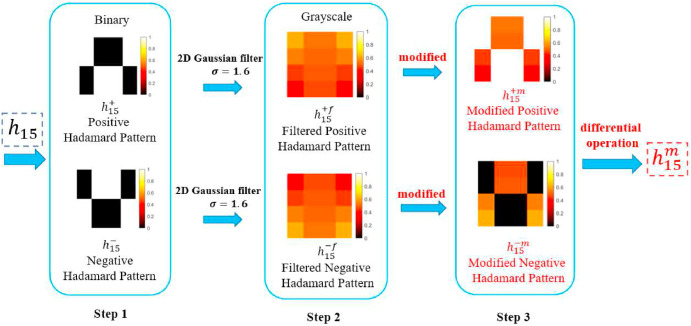
\includegraphics[width=\columnwidth]{figs/hadamard_diferencial.jpg}
\caption{Un patrón de Hadamard con valores $\pm1$ se separa en un patrón positivo y uno negativo binarios, que un DMD puede mostrar; la figura incluye además el desenfoque de la óptica (filtro gaussiano) y la combinación diferencial. \todo{citar la fuente de la figura}}
\label{fig:diferencial}
\end{figure}

\subsection{Rejilla de medición}
Hadamard exige potencias de 2, por lo que se usa una rejilla de $512\times1024$ ($N=524\,288$), cercana en píxeles a las
vistas de Tanks and Temples (979$\times$546). El cambio de relación de aspecto equivale a macropíxeles no cuadrados del
DMD y se deshace al guardar. La matriz $\mathbf{\Phi}$ no se almacena: se aplica con la transformada rápida de
Walsh-Hadamard, y $\mathbf{H}\mathbf{H}^{\top}=N\mathbf{I}$ permite que $\mathbf{\Phi}\mathbf{\Phi}^{\top}=\mathbf{I}$
tras normalizar.

\subsection{Patrones}
Las filas de Hadamard se muestran en la Fig.~\ref{fig:hadamard}. \textit{Hadamard ordenado (cake-cutting).} Se miden primero las filas con menos bloques conexos, es decir, las
frecuencias más bajas. Un patrón separable $w_i(x)w_j(y)$ tiene $(s_i+1)(s_j+1)$ bloques conexos, lo que da un orden
analítico.

\begin{figure}[t]
\centering
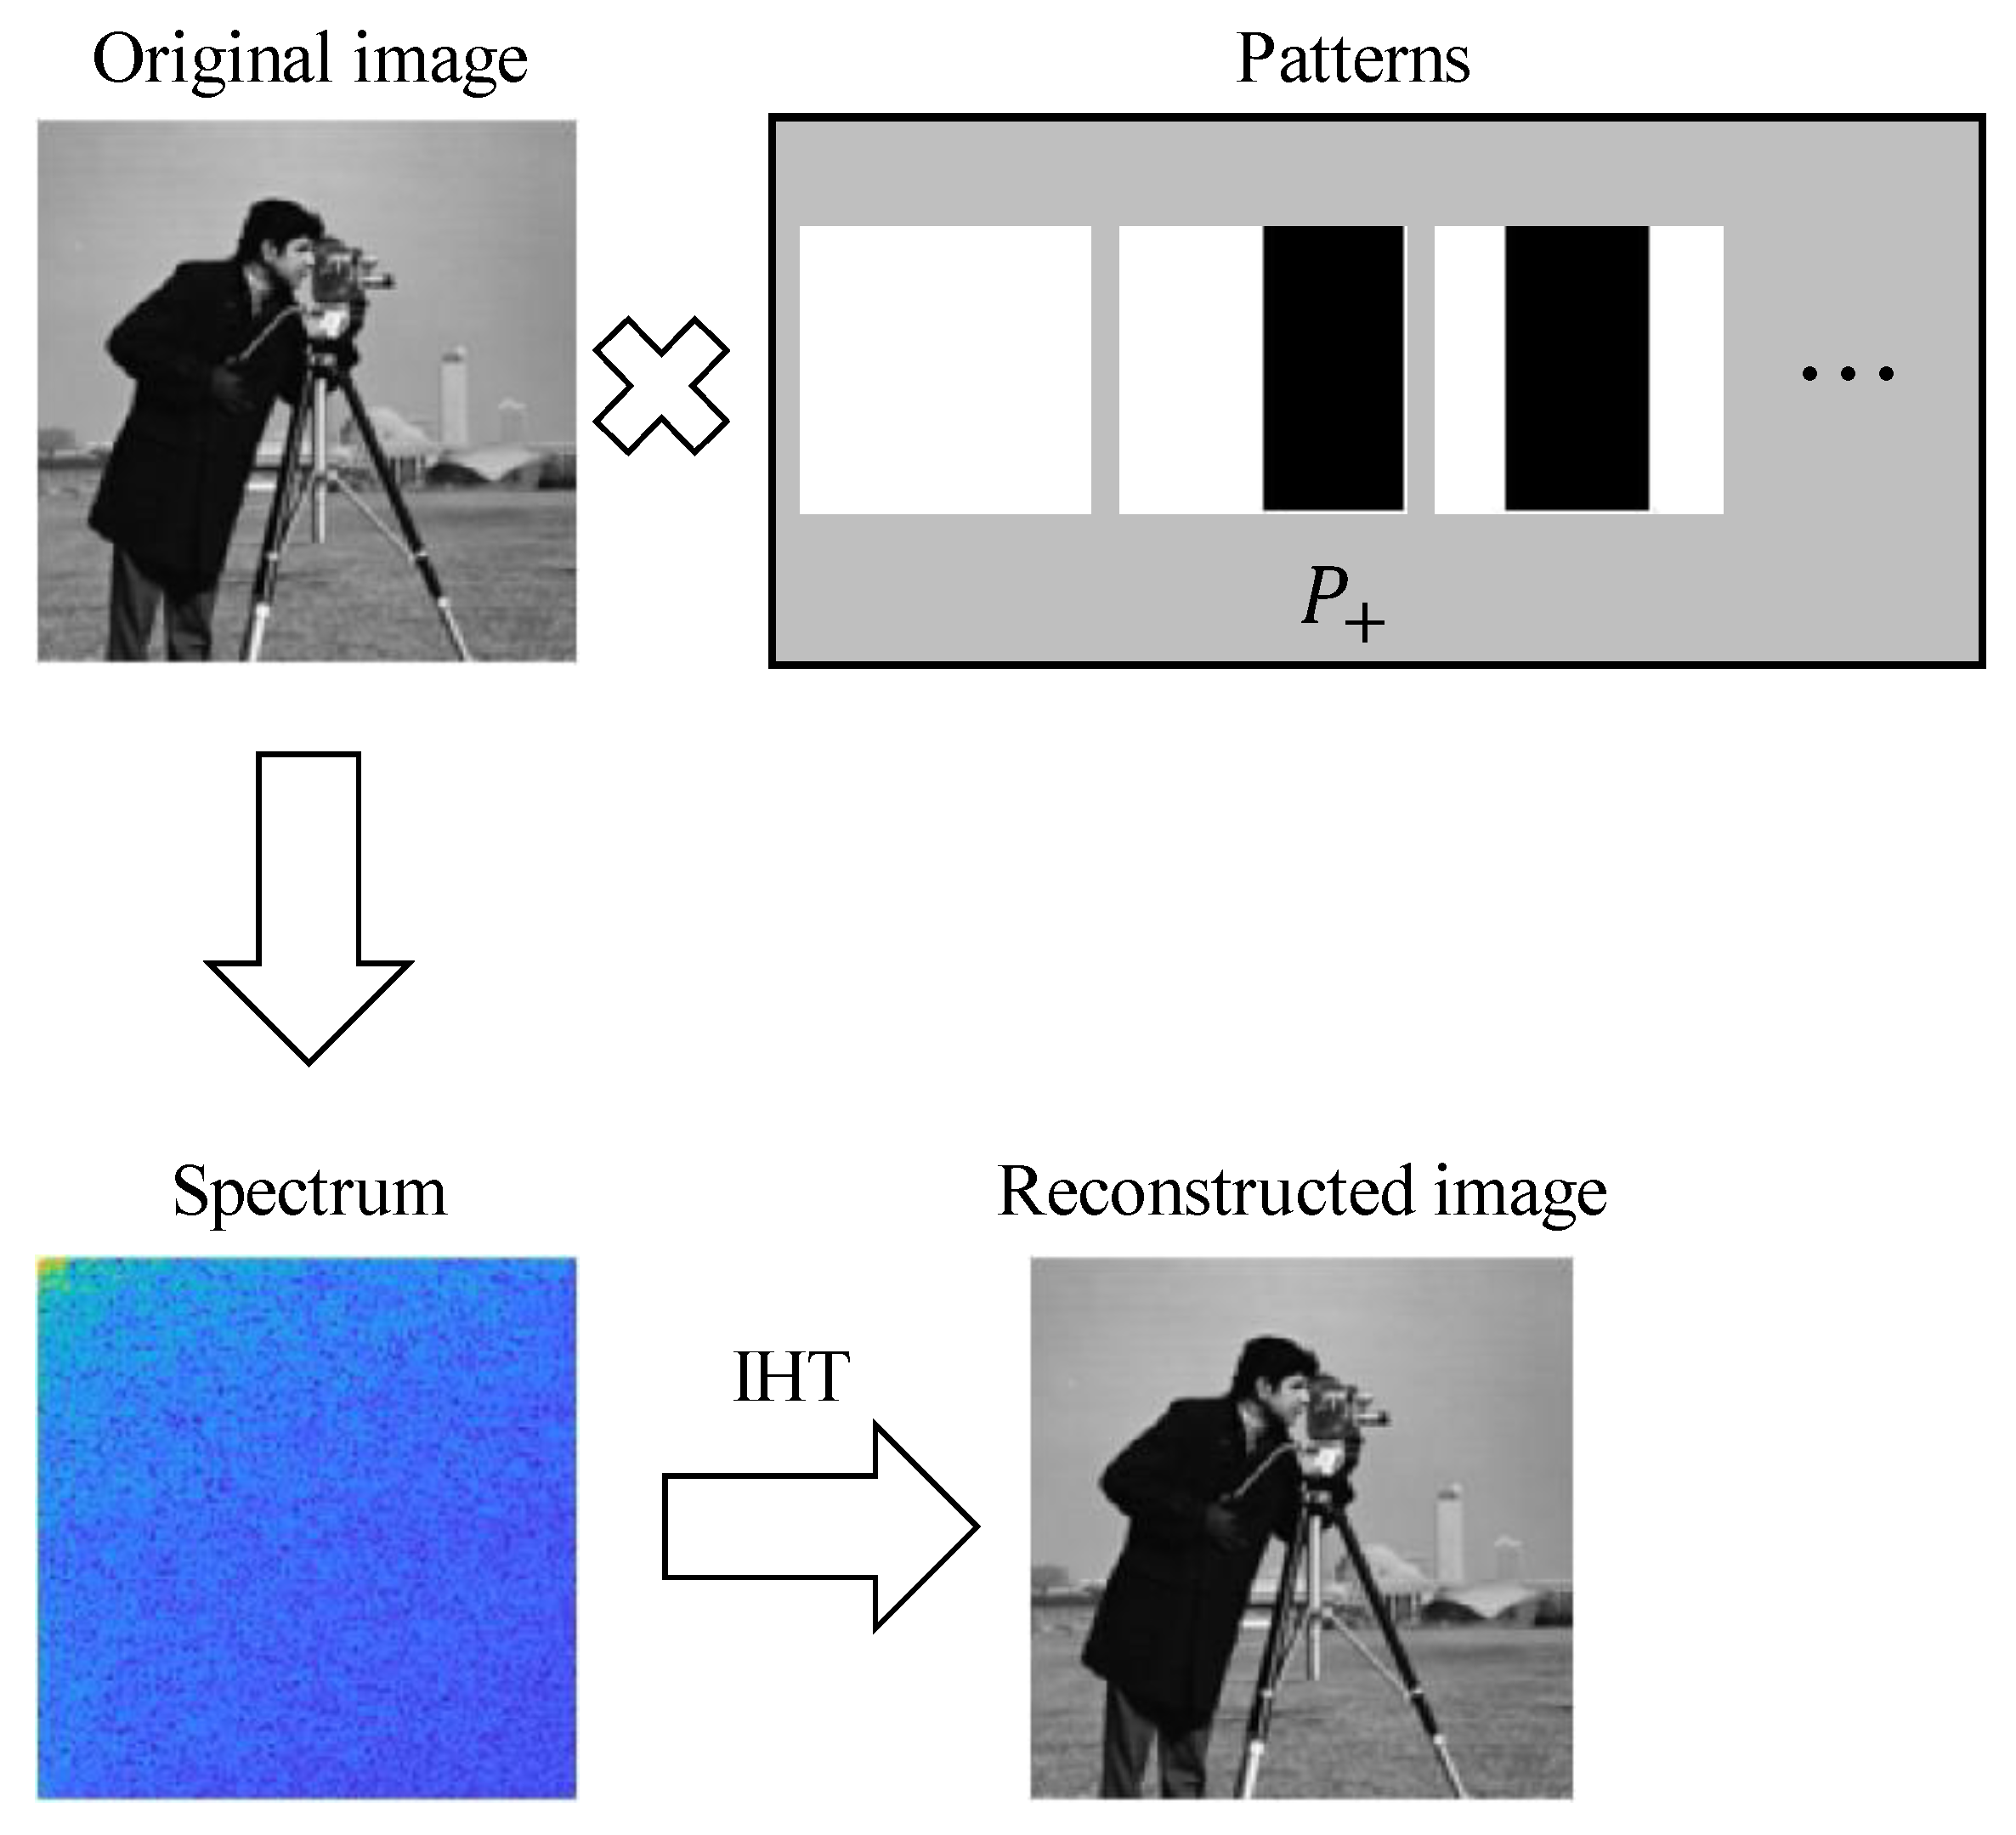
\includegraphics[width=0.8\columnwidth]{figs/Hadamard.png}
\caption{Patrones de la base de Hadamard ordenados por frecuencia. \todo{citar la fuente de la figura (material del curso)}}
\label{fig:hadamard}
\end{figure}

\textit{Binario aleatorio.} Un Bernoulli i.i.d.\ denso a $512\times1024$ ocuparía 1.7 GB al 5 \% y 17 GB al 50 \% a un
bit por entrada. Se usa una matriz estructuralmente aleatoria (permutación de píxeles, Hadamard y submuestreo). Con
una validación a baja resolución, esta matriz y un Bernoulli denso dan PSNR casi idénticos (por ejemplo 24.39 dB y
24.31 dB al 25 \%).

\subsection{Detector}
Cada medición incluye ruido de disparo de Poisson, ruido de lectura gaussiano y cuantización de $b$ bits:
\begin{equation}
y_i=Q_b\!\left(\frac{\mathrm{Pois}(\gamma\langle\mathbf{p}_i,\mathbf{x}\rangle)}{\gamma}+\mathcal{N}(0,\sigma^2)\right),
\end{equation}
con $\gamma=10^{9}$ fotones por patrón a fondo de escala, $\sigma=10^{-5}$ y $b=16$. La referencia DC se promedia 16 veces.

\section{Reconstrucción}
\subsection{Directa}
Con $\mathbf{\Phi}\mathbf{\Phi}^{\top}=\mathbf{I}$, la solución de mínima norma es
$\hat{\mathbf{x}}=\mathbf{\Phi}^{\top}\mathbf{y}$, equivalente a rellenar con ceros los coeficientes no medidos.

\subsection{Regularizada con variación total}
\begin{equation}
\hat{\mathbf{x}}=\arg\min_{\mathbf{x}}\ \tfrac12\|\mathbf{\Phi}\mathbf{x}-\mathbf{y}\|_2^2+\lambda\,\mathrm{TV}(\mathbf{x}),
\label{eq:tv}
\end{equation}
con TV isotrópica \cite{rudin1992}, resuelta con FISTA \cite{beck2009fista} y proximal de TV por FGP
\cite{beck2009tv}, con un máximo de 100 iteraciones y en lotes en GPU. El parámetro $\lambda$ se elige entre
$\{10^{-3},3\!\times\!10^{-3},10^{-2},3\!\times\!10^{-2}\}$ en cuatro vistas de entrenamiento por condición y se fija
antes de medir las demás vistas, para no sesgar la evaluación.

\section{Diseño experimental}
\subsection{Datos y condiciones}
Se usan cuatro escenas: Truck y Train (Tanks and Temples \cite{knapitsch2017}) y DrJohnson y Playroom (Deep Blending
\cite{hedman2018}), con 24 vistas equiespaciadas por escena. Las razones de medición son 5, 10, 25 y 50~\%, con dos
patrones (Hadamard ordenado y aleatorio) y dos métodos (directa y TV). Un control de solo remuestreo a la rejilla
$512\times1024$, sin SPC, aísla la pérdida que no proviene de la medición. La semilla es 449 en todas las corridas.

\subsection{Métricas}
PSNR, SSIM \cite{wang2004ssim} y LPIPS-VGG \cite{zhang2018lpips} se calculan siempre contra la imagen original a la
resolución final, con una única función para todas las condiciones.

\subsection{Implementación y recursos}
Las simulaciones se ejecutaron en una GPU NVIDIA GeForce RTX 4060 Laptop de 8~GB, con Python 3.11, PyTorch 2.11 y
CUDA 12.8. Medir una vista toma del orden de milisegundos con la transformada rápida; la reconstrucción directa tarda
entre 0.02 y 0.04~s por vista y la TV entre 0.15 y 1.3~s. Una escena completa (24 vistas, todas las condiciones y
los estudios complementarios) tarda entre 12 y 15 minutos. El código se encuentra en
\url{https://github.com/fralfaro/inf449-proyecto}.

\section{Resultados}
\subsection{Calidad frente a razón de medición}
La Fig.~\ref{fig:agregada} y la Tabla~\ref{tab:psnr} resumen la calidad media sobre las cuatro escenas. Hadamard con TV
es la mejor combinación en las tres métricas y a todas las razones: pasa de 28.05 dB y SSIM 0.798 con el 5 \% de las
mediciones a 34.63 dB y SSIM 0.914 con el 50 \%. El control de solo remuestreo alcanza 41.04 dB, que es el techo del
experimento, de modo que a razones altas la pérdida restante todavía depende de la medición.

\begin{figure*}[t]
\centering
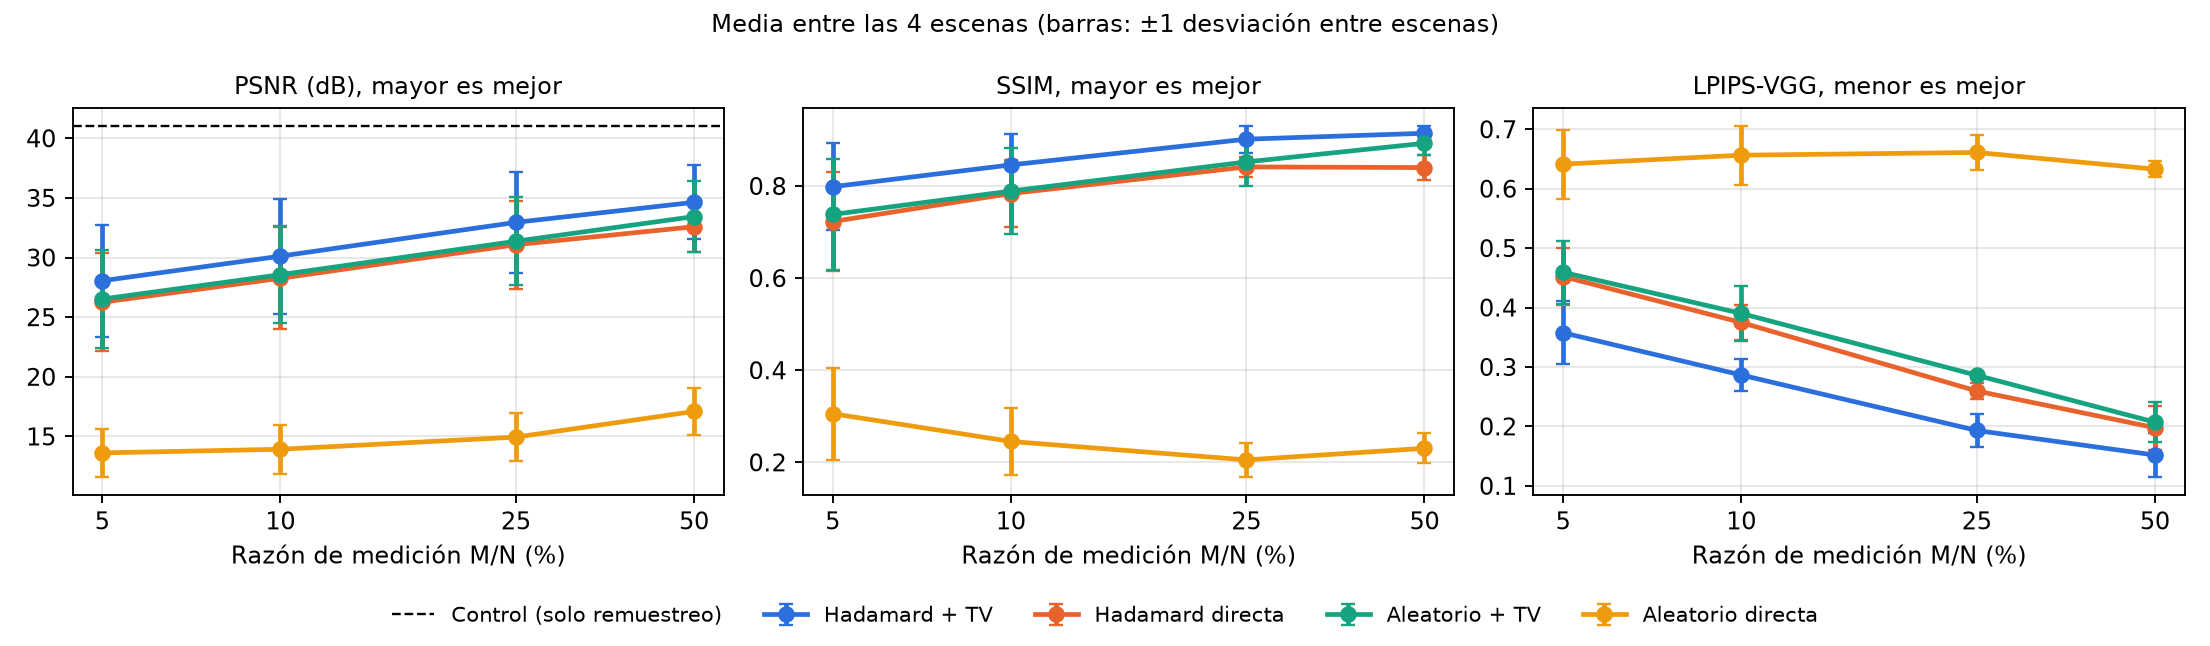
\includegraphics[width=\textwidth]{figs/fig_calidad_agregada.png}
\caption{PSNR, SSIM y LPIPS frente a la razón de medición, medias sobre las cuatro escenas (24 vistas cada una). Las
barras muestran $\pm1$ desviación entre escenas.}
\label{fig:agregada}
\end{figure*}

\begin{table}[t]
\caption{PSNR medio (dB) sobre las cuatro escenas, 24 vistas por escena.}
\label{tab:psnr}
\centering
\begin{tabular}{lcccc}
\toprule
Patrón y método & 5 \% & 10 \% & 25 \% & 50 \% \\
\midrule
Hadamard, directa & 26.25 & 28.26 & 31.07 & 32.58 \\
Hadamard, TV & \textbf{28.05} & \textbf{30.11} & \textbf{32.95} & \textbf{34.63} \\
Aleatorio, directa & 13.62 & 13.93 & 14.94 & 17.10 \\
Aleatorio, TV & 26.52 & 28.56 & 31.37 & 33.44 \\
\midrule
Control (solo remuestreo) & \multicolumn{4}{c}{41.04} \\
\bottomrule
\end{tabular}
\end{table}

\subsection{Reconstrucción directa frente a TV}
Con Hadamard, la TV mejora a la reconstrucción directa en 1.80, 1.86, 1.88 y 2.05~dB a 5, 10, 25 y 50~\%. En SSIM la
brecha crece con la razón (0.914 frente a 0.840 al 50~\%), porque la reconstrucción directa deja artefactos de bloque
que la TV suaviza. Con patrones aleatorios la reconstrucción directa no sirve (13.6 a 17.1~dB), pues los coeficientes no
medidos quedan distribuidos como ruido, y la TV la lleva a 26.5--33.4~dB. A razones altas el aleatorio con TV se acerca a
Hadamard con TV (33.44 frente a 34.63~dB al 50~\%), y la ventaja de Hadamard es mayor con pocas mediciones. La
Fig.~\ref{fig:patrones} muestra la misma medición reconstruida de cuatro formas.

\begin{figure}[t]
\centering
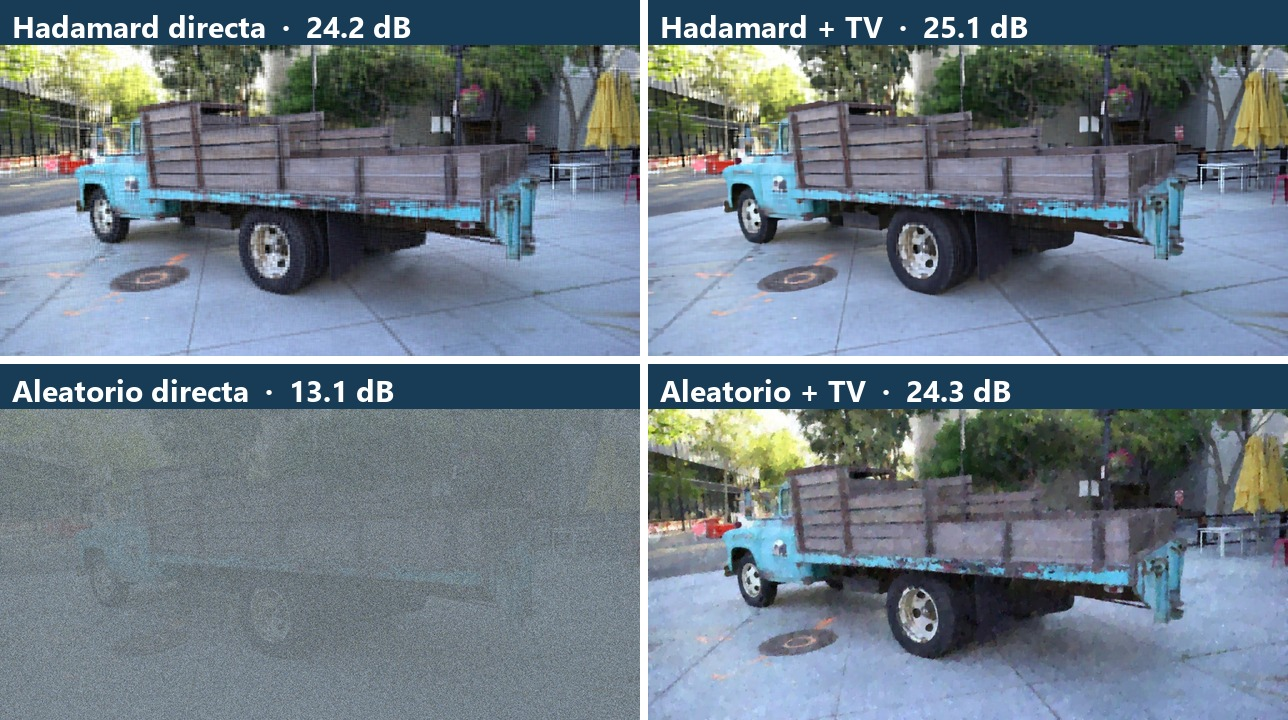
\includegraphics[width=\columnwidth]{figs/spc_patrones_truck.jpg}
\caption{Una vista de Truck al 10 \% de mediciones: Hadamard y aleatorio, con reconstrucción directa y con TV. Cada
panel indica el PSNR de esa vista.}
\label{fig:patrones}
\end{figure}

\subsection{Comparación visual}
La Fig.~\ref{fig:ratios} muestra una vista de Truck con Hadamard y TV. Con el 5 \% aparecen bloques en zonas de textura
fina, como el follaje; desde el 25 \% los bordes del camión se conservan.

\begin{figure}[t]
\centering
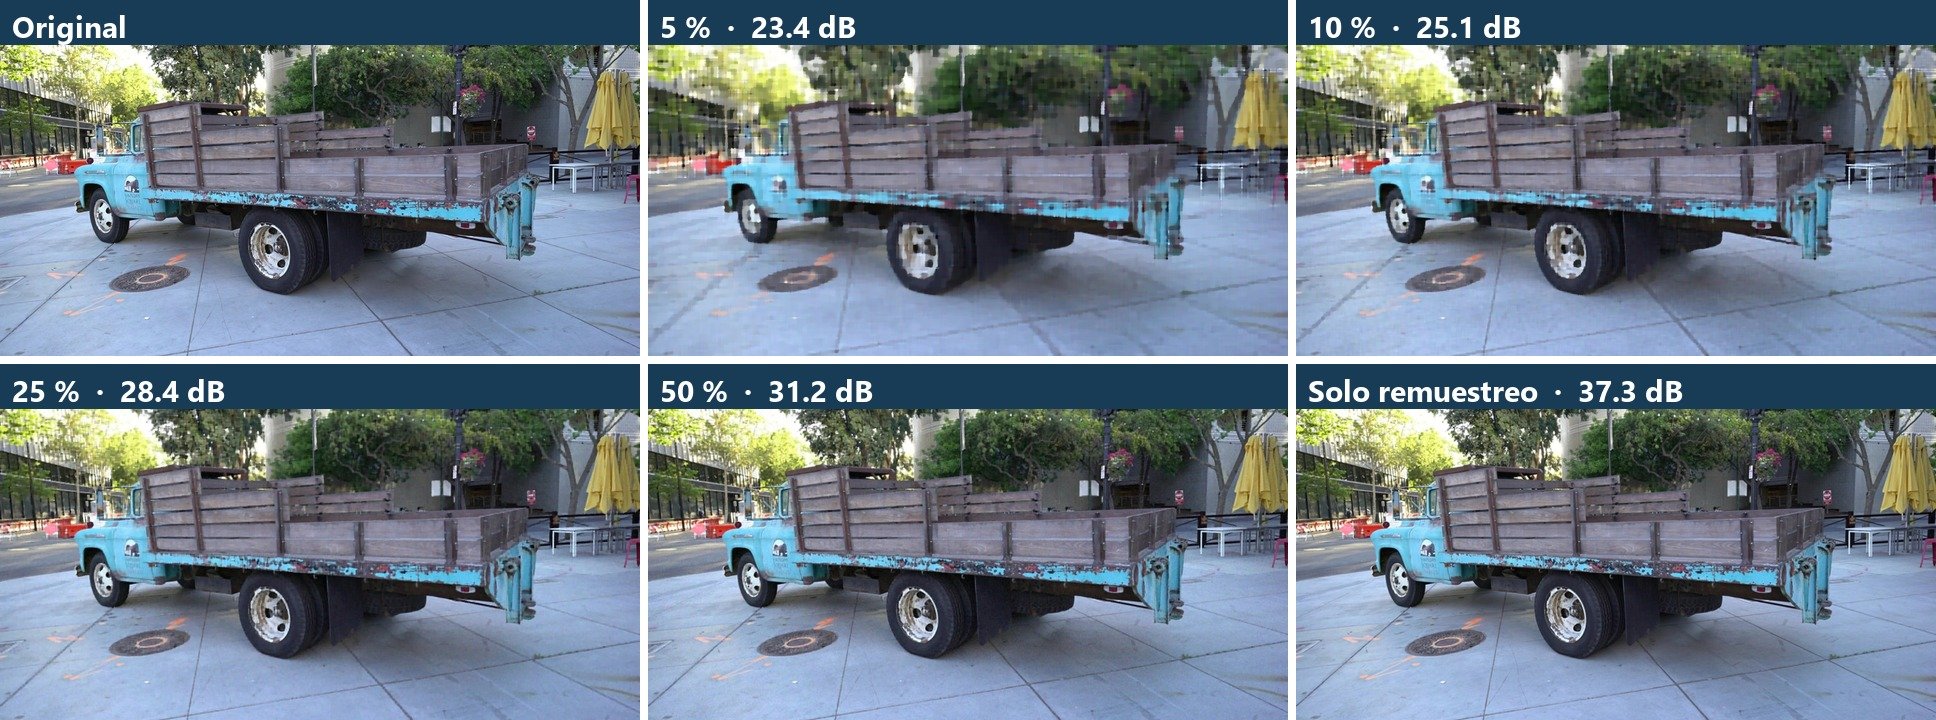
\includegraphics[width=\columnwidth]{figs/spc_ratios_truck.jpg}
\caption{Vista 000001 de Truck: original, Hadamard con TV a 5, 10, 25 y 50 \%, y control de solo remuestreo. Cada
panel indica el PSNR de esa vista.}
\label{fig:ratios}
\end{figure}

\subsection{Diferencias entre escenas}
La calidad depende más de la escena que del método: con Hadamard y TV al 5 \% el PSNR va de 23.9~dB (Train) y 24.1~dB
(Truck) a 32.6~dB (DrJohnson) y 31.5~dB (Playroom). El control de remuestreo muestra la misma separación (37.7 y 38.1~dB
frente a 44.9 y 43.5~dB). Una hipótesis, no verificada aquí, es que las escenas de Deep Blending tienen mayor resolución
nativa que la rejilla y por eso se submuestrean y suavizan, mientras que las de Tanks and Temples tienen un tamaño casi
igual al de la rejilla. Las curvas por escena están en la Fig.~\ref{fig:escenas}.

\begin{figure}[t]
\centering
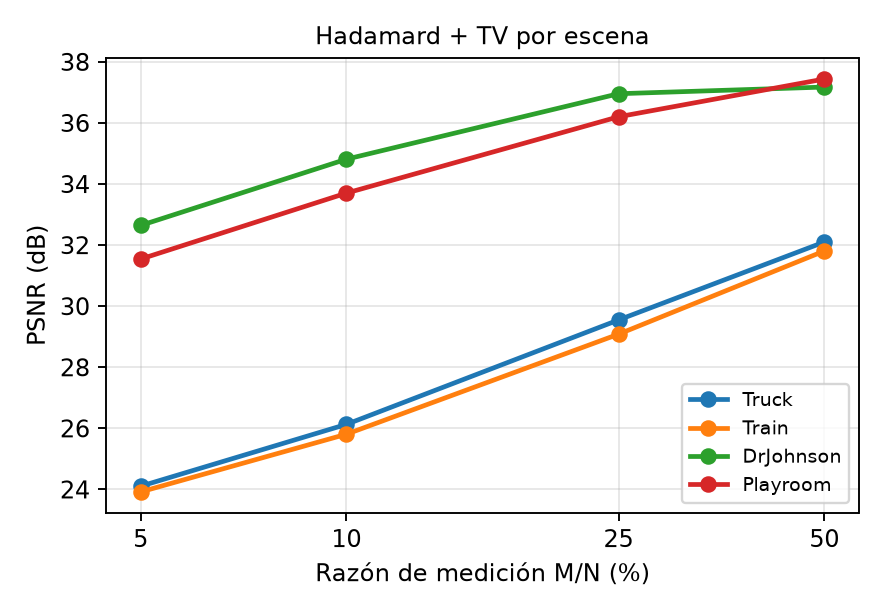
\includegraphics[width=0.85\columnwidth]{figs/fig_psnr_por_escena.png}
\caption{PSNR con Hadamard y TV, por escena.}
\label{fig:escenas}
\end{figure}

\subsection{Estudios complementarios}
Los estudios siguientes usan tres vistas de Truck al 25 \% de mediciones, de modo que son indicativos y no
estadísticamente robustos.

\textit{Ruido.} Con Hadamard y TV, el PSNR baja de 29.09~dB (detector ideal) a 28.55~dB con $10^{9}$ fotones, a
26.98~dB con $10^{8}$ y a 19.85~dB con $10^{7}$. El aleatorio con TV es más sensible: 28.85, 27.56, 25.12 y
17.72~dB. Medir en luz lineal en lugar de sRGB baja el resultado a 27.89~dB (Hadamard y TV).

\textit{Orden de los patrones.} Al 25 \% con reconstrucción directa, el orden \textit{cake-cutting} (27.27~dB) supera a
las variantes \textit{Russian dolls} (26.83~dB) y de Fourier (26.47~dB). Al 5 \% las diferencias son menores (22.40,
22.69 y 22.36~dB).

\textit{Color.} Con un presupuesto total de $0.75N$ mediciones, la medición por canal supera a la máscara Bayer con
Hadamard (27.27 frente a 25.57~dB, reconstrucción directa), pero con patrones aleatorios sin regularizar la máscara Bayer
es mucho mejor (19.49 frente a 13.62~dB). Con TV, la medición por canal es mejor con Hadamard (28.56 frente a 25.12~dB) y equivalente con aleatorio (27.56 frente a 27.39~dB).

\section{Discusión y limitaciones}
\begin{itemize}
\item Las vistas son imágenes ya capturadas, no una captura óptica: las mediciones heredan el JPEG y el desenfoque del dataset.
\item Se mide en valores sRGB y no en radiancia lineal; el estudio de ruido sugiere que la diferencia es de 0.7~dB (Hadamard y TV) a 1.9~dB (Hadamard directa).
\item La escena se asume estática durante las mediciones de cada vista.
\item Se evalúan 24 vistas en cuatro escenas; las barras de la Fig.~\ref{fig:agregada} reflejan sobre todo la variación entre escenas.
\item Los estudios de ruido, orden y color usan tres vistas de una sola escena.
\item Al pasar a 3D, las poses y la nube SfM provendrán de las imágenes originales: una SPC real no las tendría, así que
los resultados 3D serán una cota optimista.
\end{itemize}

\section{Conclusiones y trabajo futuro}
Con Hadamard ordenado y variación total se conserva una calidad media de 28.1~dB con solo el 5 \% de las mediciones y de
34.6~dB con el 50 \%, y la regularización aporta alrededor de 2~dB sobre la reconstrucción directa. Los patrones
aleatorios requieren regularización: sin ella la imagen no es utilizable, y con ella se aproximan a Hadamard solo a
razones altas. La escena influye más que el método, lo que recomienda validar con varias escenas.

Como trabajo futuro, las vistas reconstruidas alimentarán 3DGS \cite{kerbl2023} para medir cómo se propaga el error de
cada vista a la escena 3D, con una validación previa del baseline frente al artículo original. También quedan por
estimar las poses sin el GT, entrenar 3DGS directamente contra las mediciones y variar los patrones entre vistas. El
flujo ya está implementado en el repositorio.

\section*{Uso de herramientas de IA}
Durante el desarrollo se usó Claude Code de Anthropic como apoyo para explorar y revisar la implementación, organizar
la explicación y preparar visualizaciones. Las fórmulas, el código, los valores tabulados y las conclusiones fueron
contrastados por los autores con la ejecución de los notebooks y con las referencias citadas.

\bibliographystyle{IEEEtran}
\bibliography{references}

\end{document}
